
\begin{frame}
    \frametitle{}
    \begin{center}
    { {\huge 第二讲:波粒二象性}}
    \end{center}    
\end{frame}
%%%%%%%%%%%%%%%%%%%%%%%%%%%%%%%%%%
%%%%%%%%%%%%%%%%%%%%%%%%%%%%%%%%%%%%
\section{前言}
%%%%%%%%%%%%%%%%%%%%%%%%%%%%%%%%%%%%
\begin{frame}
    \frametitle{粒-波不可调和}
	\begin{columns}
		\begin{column}[t]{0.46\linewidth}
			粒子的特性
			\begin{itemize}
				\item 确定的位置、能量、动量等
				\item 两个粒子不能同时占据同一位置
				\item 同一粒子也不能同时占据多个位置
				\item 会产生碰撞现象
			\end{itemize}
		\end{column}
		\begin{column}[t]{0.46\linewidth}
			波的特性
			\vspace{1ex}
			\begin{itemize}
				\item 确定的波长、振幅、相位等
				\item 可以同时出现在同一位置
				\item 可以同时占据多个位置
				\item 衍射及干涉,不碰撞
			\end{itemize}
		\end{column}
	\end{columns}
\end{frame}

\begin{frame} 
    \begin{center}
        \includegraphics[width=0.6\textwidth]{figs/2021-12-02-15-26-40.png}
    \end{center}
    \begin{itemize}
        \item 一个物体要么是粒子,要么是波
        \item 通过上述特性进行判定
        \item 这个方法一直是有效的
        \item 但有时却无效, 比如说: **光** 
    \end{itemize}
\end{frame}

\begin{frame}
	\begin{columns}
		\begin{column}[t]{0.46\linewidth}
            水波
            \begin{center}
                \includegraphics[width=2.5in,height=2.5in]{figs/2021-12-02-15-46-16.png}
            \end{center}
		\end{column}
		\begin{column}[t]{0.46\linewidth}
            光波
            \begin{center}
                \includegraphics[width=2.5in,height=2.5in]{figs/2021-12-02-15-49-36.png}
            \end{center}
		\end{column}
	\end{columns}
\end{frame}

\begin{frame} 
    \begin{center}
        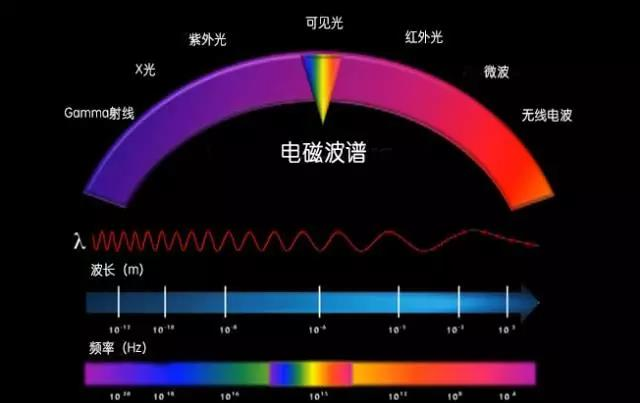
\includegraphics[width=0.75\textwidth]{figs/2021-12-02-16-23-16.png}
    \end{center}
    光只是一定波长范围内的电磁波
\end{frame}

\begin{frame} 
    光的波动说面临的困难:
    \begin{itemize}
        \item 黑体辐射
        \item 光电效应
        \item 康普顿效应
        \item 氢原子光谱
    \end{itemize}
\end{frame}

%%%%%%%%%%%%%%%%%%%%%%%%%%%%%%%%%%%%
\section{光电效应}
%%%%%%%%%%%%%%%%%%%%%%%%%%%%%%%%%%%%
\begin{frame} 
    \frametitle{光电效应实验}   
    \begin{center}
       \includegraphics[width=0.53\textwidth]{figs/2021-12-02-16-01-21.png}
   \end{center}  
   \bullet 具有瞬时性 \\
   \bullet 存在临界频率 $\nu_0$ \\
   \bullet 光电子能量与光的频率决定
\end{frame}  

\begin{frame} 
    In 1905, Einstein considered the derivation of Planck's Law  \\
    \begin{itemize}
        \item Plank’s Law was consistent with experment but not with existing theory
        \item Rayleigh-Jeans Law was consistent with existing theory but not with experiment
        \item For treating Ultraviolet Catastrophe, he proposed the light quantum hypothesis
        \item Using light quantum hypothesis, he explained the Photoelectric effect
    \end{itemize}
\end{frame}

\begin{frame}  
    \frametitle{光量子假说}  
    \begin{center}
        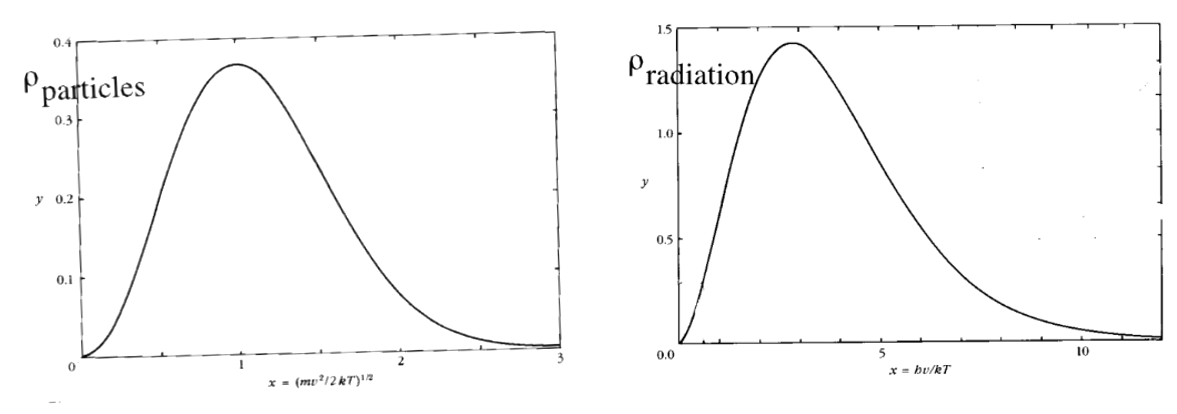
\includegraphics[width=0.6\textwidth]{figs/mbd.png}
    \end{center}
    \begin{tcolorbox}[colback=yellow!10,colframe=red!75!black,title=]
        \bullet Light likes particles with unit energy $h\nu$ (quanta).\\  
        \bullet The energy of n light quantum is $nh\nu$. \\
        \bullet The momentum of light quantum is (1918)
        \[p=\frac{E}{c}=\frac{h\nu}{c}=\frac{h}{\lambda}\]
    \end{tcolorbox}
\end{frame}



\begin{frame} 
    基于光量子假说,爱因斯坦提出一个光电效应公式
    $$
    \frac{1}{2}m_eV_0^2=h\nu-W
    $$
    \begin{itemize}
        \item 瞬时性:光子碰上电子时,能量被瞬时吸收
        \item 临界频率:$\nu_0=\frac{W}{h} $
        \item 光电子能量与光的频率决定: $E_k=h\nu-W$
    \end{itemize}
    {\color{deepred} Nobel Prize in physics(1921)}
\end{frame}

\begin{frame} 
    基于光电效应公式:
$$
\frac{1}{2}m_eV_0^2=h\nu-W
$$
1916年,密立根实验上测定普朗克系数,验证光子说\\
1923年诺贝尔物理学奖 
\end{frame}

\begin{frame} 
    \begin{tcolorbox}[colback=yellow!10,colframe=red!75!black,title=意义:]
        \begin{itemize}
            \item 揭示能量子的本质:在于光本身是量子化的,具有粒子性
            \item 揭示光的本质:光既具波动性又具粒子性。
        \end{itemize}
    \end{tcolorbox}
    \begin{tcolorbox}[colback=yellow!10,colframe=red!20!black,title=普朗克的评价:]
    在近代物理学结出硕果的那些重大问题中,很难找到一个问题是爱因斯坦没有做过重要贡献。
    在他的各种推测中,他有时可能也曾经没有中标的。例如他的光量子假设,就有点迷失了方向 
    \end{tcolorbox}
\end{frame}

%%%%%%%%%%%%%%%%%%%%%%%%%%%
\section{康普顿效应}
%%%%%%%%%%%%%%%%%%%%%%%%%%%%%%%%%%%%

\begin{frame}   
    \frametitle{康普顿效应 (1922)}
    \begin{center}
        \includegraphics[width=0.8\textwidth]{figs/compton.png}
    \end{center}  
    经验公式:$\lambda_{out}-\lambda_{in}=\lambda_e(1-\cos \theta)$
\end{frame}

\begin{frame}  
    \frametitle{推导经验公式} 
    Energy of electron 
    \begin{equation*}
        E^2 =m_ec^2=p^2c^2 +m_0 ^2 c^4 
    \end{equation*}
    Energy of light quantum
    \begin{equation*}
        E =pc 
    \end{equation*}
    energy conservation law
    \begin{equation*}
        \begin{split}
        E_i + m_0 c^2 &= E_o + m_ec^2 \\
        (E_i -E_o + m_0 c^2)^2 &= E_e ^2\\
        (p_i c-p_o c + m_0 c^2) ^2 &= p_e ^2 c^2 +m_0 ^2 c^4 \\
        (p_i-p_o)^2 +2 m_0 (p_i c-p_o c) &= p_e ^2
    \end{split}
    \end{equation*}
\end{frame}

\begin{frame}  
    momentum conservation law
    \begin{equation*}
        \begin{split}
            \vec{p}_i -\vec{p}_o &= \vec{p}_e \\
            (\vec{p}_i -\vec{p}_o)\cdot (\vec{p}_i -\vec{p}_o)  &= \vec{p}_e\cdot \vec{p}_e   \\
            p_i ^2 + p_o ^2 -2p_i p_o \cos \theta &= p_e ^2  \\
            p_i ^2 + p_o ^2 -2p_i p_o \cos \theta &= (p_i-p_o)^2 +2 m_0 (p_i c-p_o c) \\
            \frac{1}{p_o} -\frac{1}{p_i} &= \frac{1}{m_0 c} (1-\cos \theta) \\
            \lambda_o -\lambda_i &= \frac{h}{m_0 c} (1-\cos \theta) 
        \end{split}
    \end{equation*}
\end{frame}

\begin{frame}   
    \begin{tcolorbox}[colback=yellow!10,colframe=red!75!black,title=Significance]
        \bullet The light of wavelength \lambda possesses quantum momentum \[p=\frac{h}{\lambda}\]
        \bullet Momentum conservation law works in subatom scales 
    \end{tcolorbox}   
    {\color{deepred} Nobel Prize in physics(1927)}\\
\end{frame}

%%%%%%%%%%%%%%%%%%%%%%%%%%
\section{氢原子光谱}
%%%%%%%%%%%%%%%%%%%%%%%%%%%%%%%%%%%%
\begin{frame}  
     \frametitle{氢原子光谱}
     \begin{center}
        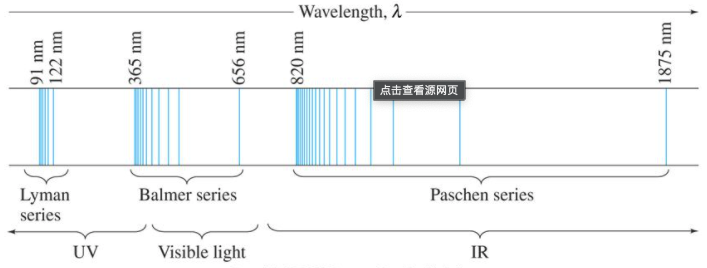
\includegraphics[width=0.8\textwidth]{figs/hydspe.png}
    \end{center}  
    经验公式:
       $\dfrac{1}{\lambda}=R_H c (\dfrac{1}{m^2} -\dfrac{1}{n^2})$ \\
    \alert{Problem:} the formula cannot be derived from existing theory
\end{frame}

\begin{frame} 
    \frametitle{Rutherford model}  
    \begin{center}
        \includegraphics[width=0.8\textwidth]{figs/utherford_atom.png}
    \end{center}  
\end{frame}

\begin{frame}   
    \frametitle{Bohr's model}  
    \begin{center}
        \includegraphics[width=0.6\textwidth]{figs/bohratom.png}
    \end{center}  
    1905年爱因斯坦提出的光子概念,不受名人的重视,普朗克把爱因斯坦的光量子概念说成是“迷失了方向”。
    1913年,28岁的玻尔,创造性地把光子概念用到卢瑟福模型上,成功破解氢原子光谱问题 
\end{frame}

\begin{frame}  
    \begin{tcolorbox}[colback=yellow!10,colframe=red!75!black,title=]
    Bohr asummed that :\\
    ~\\
    \bullet Stationary states: Electrons move around the nucleus only in certain allowed circular orbits with fixed energy \\
    \[ L=n \frac{h}{2\pi}= n \hbar,\qquad (\oint p_i dq_i = n_i h)\]
    \bullet Quantum transition: Electron can jump between stationary state orbits when absorbed or emitted a photon with certain energy\\
    \[ h\nu=E_n -E_m \]
    \end{tcolorbox}
\end{frame}

\begin{frame}   
    \frametitle{推导光谱公式}
    \bullet Stationary state orbit radius:
    \begin{equation*}
        \begin{split}
            m\frac{v^2}{r}&=\frac{1}{4\pi\epsilon_0} \frac{e^2}{r^2} \\
            L=&mvr =n\hbar \\
            r_n&= n^2 (\frac{\epsilon_0 h^2}{m\pi e^2}) =n^2 r_1   
        \end{split} 
     \end{equation*}
     \bullet Stationary state orbit energy: 
     \begin{equation*}
        \begin{split}
            E_n &= T + U \\
            &= \frac{1}{2}mv^2- \frac{1}{4\pi\epsilon_0} \frac{e^2}{r_n ^2} \\
            &= \frac{1}{n^2} (-\frac{m e^4}{8 \epsilon_0 ^2 h^2}) = \frac{E_1}{n^2}
        \end{split}  
     \end{equation*}
\end{frame}

\begin{frame}
    \bullet Spectrum formula: 
    \begin{equation*}
        \begin{split}
         \nu&=\frac{E_n -E_m}{h} \\
         &= \frac{m e^4}{4\pi \hbar ^3} [\frac{1}{m^2} -\frac{1}{n^2}]
        \end{split}  
     \end{equation*}
     \bullet Rydberg constant : 
     \[R_{theo}= \frac{m e^4}{4\pi \hbar ^3 c} =1.0973731\times 10^7 m^{-1}\]
    \[R_{exp}=1.0974\times10^7 m^{-1} \]  
    {\color{deepred} Nobel Prize in physics(1922)}\\ 
\end{frame}

\section{光的波粒二象性}  
\begin{frame} 
  \frametitle{光的波粒二象性}  
  \bullet In 1905, when Einstein first put forward this hypothesis, 
  he simply stated that light consisted of quanta with energy \[ E = hν \] 
  \bullet In 1917, he stated that the light quantum carried a momentum of  \[ p=\frac{h}{\lambda}\]
  At this point, the light quantum with massless particle property was named as photon (光子)
\end{frame}

\begin{frame}  
  $\begin{cases}
    \text{Light behaves like waves }\\
    \text{~~\qquad Interference} \\
    \text{~~\qquad Diffraction} \\
    \text{Light behaves like particles}\\
    \text{~~\qquad Black body radiation} \\
    \text{~~\qquad Photoelectric effect} \\
    \text{~~\qquad Compton effect} \\
   \end{cases}$\\
   ~~\\
   Light has both wave and particle properties is called \alert{wave-particle duality} of light
\end{frame}



%%%%%%%%%%%%%%%%%%%%%%%%%%%
\section{物质波假说}
%%%%%%%%%%%%%%%%%%%%%%%%%%%%%%%%%%%%

\begin{frame}   
  \frametitle{物质波假说}
  \begin{tcolorbox}[colback=yellow!10,colframe=red!75!black,title=]
  In 1923, de Broglie states that if light which is classically a wave could behave as a particle, 
  then classical particles could also behave as quantum waves.
  \[\lambda=\frac{h}{p}\]
  \[\nu =\frac{E}{h}\]
  \end{tcolorbox}
\end{frame}

\begin{frame}  
    \frame{}
    De Broglie wavelength of the electron in Bohr's atom model
    \begin{equation*}
        \begin{split}
            L&=n\hbar \\
            r \cdot p & =  n\frac{h}{2 \pi} \\
            2\pi r&=  n\frac{h}{p}\\
            2\pi r&=  n\lambda 
        \end{split} 
     \end{equation*}
     Called standing-wave condition 
\end{frame}


\begin{frame}   
  \frametitle{Experimental verification}
  \begin{center}
    \includegraphics[width=0.5\textwidth]{figs/elediffr.jpeg} \\
    Electron diffraction patterns (Davisson and Germer, 1927)
\end{center} 
\end{frame}
\begin{frame}   
    \begin{center}
      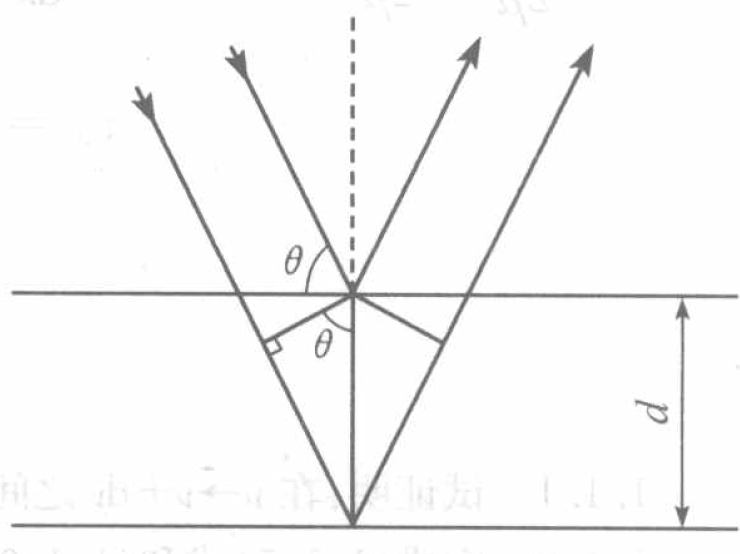
\includegraphics[width=0.6\textwidth]{figs/scatting.png} \\
    \end{center} 
    \begin{itemize}
        \item Meeting Bragg formula $2d\sin \theta=n\lambda $
        \item Obtaining the wavelength of electron (about 0.16X $nm$), agreeing well with the 
   calculated de Broglie wavelength 
    \end{itemize}
  {\color{deepred} Nobel Prize in physics(1937)}  
  \end{frame}

\begin{frame} 
    \begin{tcolorbox}[colback=yellow!10,colframe=red!75!black,title=]
        Extended the wave-particle duality from light to particles! \\
        {\color{deepred} Nobel Prize in physics(1929)} for discovery of wave nature of electrons
    \end{tcolorbox}  
\end{frame}

\begin{frame}{电子双缝干涉实验}
    \includemedia[
    width=1.0\linewidth,height=0.67\linewidth, % 16:9
    activate=pageopen,
    addresource=figs/doubleslite-n.mp4,
    flashvars={
    source=figs/doubleslite-n.mp4
    &autoPlay=true % start playing on activation
    &loop=true
    }
    ]{}{VPlayer.swf}
\end{frame}

\begin{frame}  
    \begin{tcolorbox}[colback=yellow!10,colframe=red!75!black,title=Conclusion]
    Wave-particle duality is the inherent attribute of matter
    \end{tcolorbox} 
\end{frame}

\begin{frame}  
    \frametitle{Big problems} 
  \begin{center}
    How we can interpret a world where waves are particles and particles are waves
  \end{center} 
\end{frame}

\begin{frame}  
  \begin{center}
    The answer is \alert{Quantum Mechanics}
  \end{center} 
\end{frame}

\begin{frame}   
    \frametitle{学术讨论}
    \begin{center} 
    {\color{red} \Large How can something be both a particle and a wave?}\\
    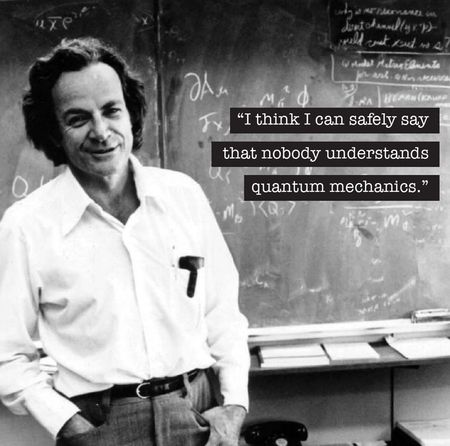
\includegraphics[width=0.4\textwidth]{figs/noone.jpg}
  \end{center} 
\end{frame}
